\chapter{EFT-Modell mit MG5}
In diesem Kapitel erfolgt eine Variation der Wilson-Koeffizienten mit Hilfe eines EFT Modells für MG. Dies ermöglicht die Berechnung eines Modells der Wirkungsquerschnitte für den EFTfitter mit dessen Hilfe später die Wilson-Koeffizienten bestimmt werden können.

\section{Zusammensetzung des Wirkungsquerschnitts}
Der Fit des EFTfitters basiert auf einem funktionellen Zusammenhang zwischen den Observablen, in diesem Fall den Wirkungsquerschnitten, und den Operatoren höherer Ordnung. Diese Abhängigkeit wird durch das implementierte Modell und dem entsprechend mit der Likelihood ausgedrückt.\\
Für die Berechnung des Wirkungsquerschnitts werden alle zugehörigen Feynman-Graphen, sowohl die des SM, als auch die der EFT-Operatoren, betrachtet. Daher ergibt sich der Wirkungsquerschnitt zu:
\begin{align}
  \sigma = \sigma_{SM} + \frac{1}{\Lambda^2} \sum_{i} C_i \sigma_i^\text{interf.} + \frac{1}{\Lambda^4} \sum_{i \leq j} C_i C_j \sigma_{ij}^\text{BSM} + \mathcal{O} \left(\frac{1}{\Lambda^6}\right).
\end{align}
Die einzelnen Wirkungsquerschnitte $\sigma_i$ besitzen eine quadratische Abhängigkeit von den Wilson-Koeffizienten $C_i$ und die BSM-Beiträge in führender Ordnung ergeben sich durch die Interferenz zwischen dem SM und der BSM-Physik. Dies liegt unter Anderem daran, dass die Beiträge durch die Interferenz zwischen den BSM-Physik-Beiträgen untereinander mit $\frac{1}{\Lambda^4}$ unterdrückt sind. Um trotzdem ein möglichst genaues Modell für die Abhängigkeit der Wirkungsquerschnitte von den Wilson-Koeffizienten zu erhalten, müssen auch diese Beiträge betrachtet werden. Dies wurde bereits in dem Papier\cite{Wilson-Beiträge} untersucht. Zur Bestimmung des Modells ist es zudem notwendig die Wirkungsquerschnitte für verschiedene Konfigurationen der Wilson-Koeffizienten zu bestimmen.

\section{Variation der Wilson-Koeffizienten mit MadGraph5}
Eine Möglichkeit die Wilson-Koeffizienten zu variieren ist mit Hilfe eines MG Modells, dass Operatoren der Massendimension sechs enthält und damit eine Berechnung der Wirkungsquerschnitte unter dem Einfluss dieser ermöglicht. Dazu wird in MadGraph5 das TEFT\_EF UFO Modell\cite{EFTModell} eingebunden. Dies erlaubt NLO Rechnung in der QCD und enthält alle für die Top-Quark-Physik relevanten Operatoren der Dimension sechs.
Die Berechnung erfolgt mit dem genannten Modell in NLO in QCD unter der Verwendung des $\text{CTEQ}6\text{L}1$ PDF Sets. Zudem wird die Energieskala auf $\SI{1}{\tera\electronvolt}$ festgelegt. Unter diesen Vorraussetzungen wird der Prozess $pp~\rightarrow~t\bar{t}~\gamma$ mit den von ATLAS genutzten Schnitten implementiert.\\
Da die Berechnung statistische Unsicherheiten enthält, bietet es sich an anstatt nur genügend viele Berechnungen der Monte Carlo Wirkungsquerschnitte $\sigma_{MC}$ für ein bestimmtes Gleichungssystem zur Bestimmung der Wirkungsquerschnitte $\sigma_i$ durchzuführen sondern mehr. Zudem werden genauere Ergebnisse erhalten, wenn sowohl Berechnungen bei denen nur ein Wilson-Koeffizient angeschaltet ist, als auch welche beidenen mehrere oder sogar alle betrachtet werden, getätigt werden.\\
Die berechneten Monte Carlo Wirkungsquerschnitte:
\begin{align}
  \sigma_{MC}({C_i}) = \sigma_{SM} + \sum_{i} C_i \frac{\sigma_i}{\Lambda^2} + \sum_{i \leq j} C_i C_j \frac{\sigma_{ij}}{\Lambda^4} + \mathcal{O}(\frac{1}{\Lambda^6})
\end{align}
bilden die Stützstellen zur späteren Bestimmung der gesuchten Wirkungsquerschnitte. Mit Hilfe des Vakuumerwartungswert des Higgs $\SI{246}{\giga\electronvolt}$ und der Wahl $\Lambda = \SI{1}{\tera\electronvolt}$ lassen sich die $\sigma_{MC}$ in natürliche Einheiten umrechnen. Unter Vernachlässigung de Terme der Ordnung $\mathcal{O}(\frac{1}{\Lambda^6})$ ergeben sie sich zu:
\begin{align}
  \sigma_{MC}({\tilde{C_i}}) \approx \bar{\sigma}_{SM} + \sum_{i} \tilde{C_i} \bar{\sigma_i} + \sum_{i \leq j} \tilde{C_i} \tilde{C_j} \bar{\sigma}_{ij}.
\end{align}
Hierbei sind die $\tilde{C}_i = \frac{v^2}{\Lambda^2} C_i$.
Bei der Berechnung des $t\bar{t}\gamma$ Produktionswirkungsquerschnitts können, wie in Kapitel~\ref{top} bereits erwähnt, die Operatoren $O_{tG}$, $O_{tW}$ und $O_{tB}$ beitragen. Damit ergibt sich die Interpolationsfunktion zu:
\begin{align}
  \sigma_{t\bar{t}\gamma, MC}({\tilde{C}_{tG}, \tilde{C}_{tW}, \tilde{C}_{tB}}) = \bar{\sigma}_{SM} + \tilde{C}_{tG}\bar{\sigma}_{tG} + \tilde{C}_{tW}\bar{\sigma}_{tW} + \tilde{C}_{tB}\bar{\sigma}_{tB}\\
  + \tilde{C}_{tG}^2\bar{\sigma}_{tGtG} + \tilde{C}_{tW}^2\bar{\sigma}_{tWtW} + \tilde{C}_{tB}^2\bar{\sigma}_{tBtB}\\
  + \tilde{C}_{tG} \tilde{C}_{tW}\bar{\sigma}_{tGtW} + \tilde{C}_{tG} \tilde{C}_{tB}\bar{\sigma}_{tGtB} + \tilde{C}_{tW} \tilde{C}_{tB}\bar{\sigma}_{tWtB}
\end{align}
und es müssen insgesamt zehn Parameter $\bar{\sigma_i}$ und $\bar{\sigma}_{ij}$ bestimmt werden. Dazu werden die Wilson-Koeffizienten $C_{tG}$, $C_{tW}$ und $C_tB$ im Bereich $[-30~,~30]$ variiert. Um erneut nur die semileptonischen Endzustände zu betrachten, müssen auch in diesem Fall die $\sigma_{t\bar{t}\gamma, MC}$ mit dem $\mathrm{BR} = \SI{30}{\percent}$ multipliziert werden. Aus diesen Berechnungen lassen sich dann mit der Methode der kleinsten Quadrate die gesuchten Parameter bestimmen, aus denen sich schließlich das Modell für den EFTfitter ergibt.

\section{Schnitte mit der Hypereben zur Bestimmung der gesuchten Parameter}
Die Schnitte mit der sich ergebenen Hyperebene sind parabelförmig, wenn nur ein Wilson-Koeffizient variiert wird. Dies ist zu erwarten, da die Zusammensetzung der Monte Carlo Wirkungsquerschnitt in der höchsten Potenz aus quadratischen Anteilen besteht. Die direkt an der Photonabstrahlung beteiligten Wilson-Koeffizienten $C_{tW}$ und $C_{tB}$ folgen ziemlich genau diesem parabelförmigen Verlauf. Dies ist in Abbildung~\ref{fig:WtW} und~\ref{fig:WtB} veranschaulicht. Lediglich die berechneten Wirkungsquerschnitte für den Wilson-Koeffizienten $C_{tG}$ weisen stärke Abweichungen auf, dies ist in Abbildung~\ref{fig:WtG} dargestellt.\\
Dies liegt vermutlich daran, dass der Wertebereich der berechneten Wirkungsquerschnitte deutlich größer ist. Dadurch sind größere Abweichung plausibel, die ebenfalls größere Unsicherheiten mit sich bringen. Da es sich bei dem Schnitt nur um einen kleinen Bereich handelt, führt dies zudem zu einer größeren Unsicherheit, dadurch das der Schnitt mit einer sehr hochdimensionalen Ebene erfolgt. Die Abweichungen könnten verbessert werden, indem zum einen mehr Stützstellen berechnet werden  und eine genauere Rechnung erfolgt.\\
Zudem liegen die Wilson-Koeffizienten auf Grund der Wahl der natürlichen Einheiten im Bereich $[-2~,~2]$.
\begin{figure}
  \begin{subfigure}[c]{0.5\textwidth}
    \centering
    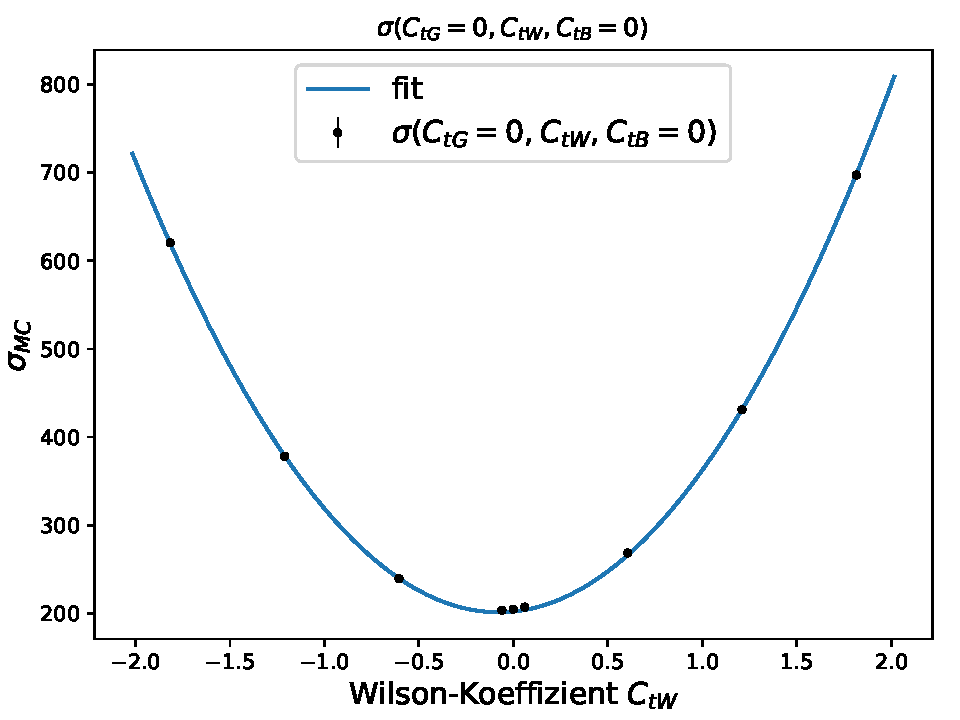
\includegraphics[width=\textwidth]{Plots/combi_plot_tW.pdf}
    \subcaption{Verlauf für $C_tW$ mit $C_{tB}=C_{tG}=0$.}
    \label{fig:WtW}
  \end{subfigure}
  \begin{subfigure}[c]{0.5\textwidth}
    \centering
    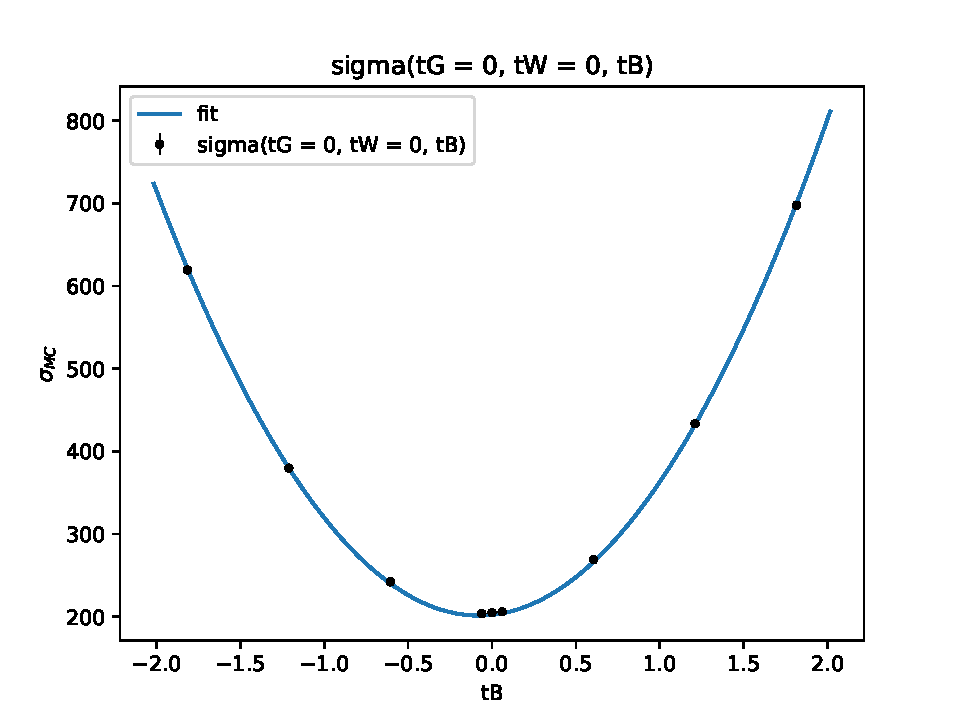
\includegraphics[width=\textwidth]{Plots/combi_plot_tB.pdf}
    \subcaption{Verlauf für $C_tB$ mit $C_{tW}=C_{tG}=0$.}
    \label{fig:WtB}
  \end{subfigure}
  \caption{Graphische Darstellung des parabelförmigen Verlaufs der Wirkungsquerschnitte für die Betrachtung einzelner Wilson-Koeffizienten.}
\end{figure}
\begin{figure}
  \centering
  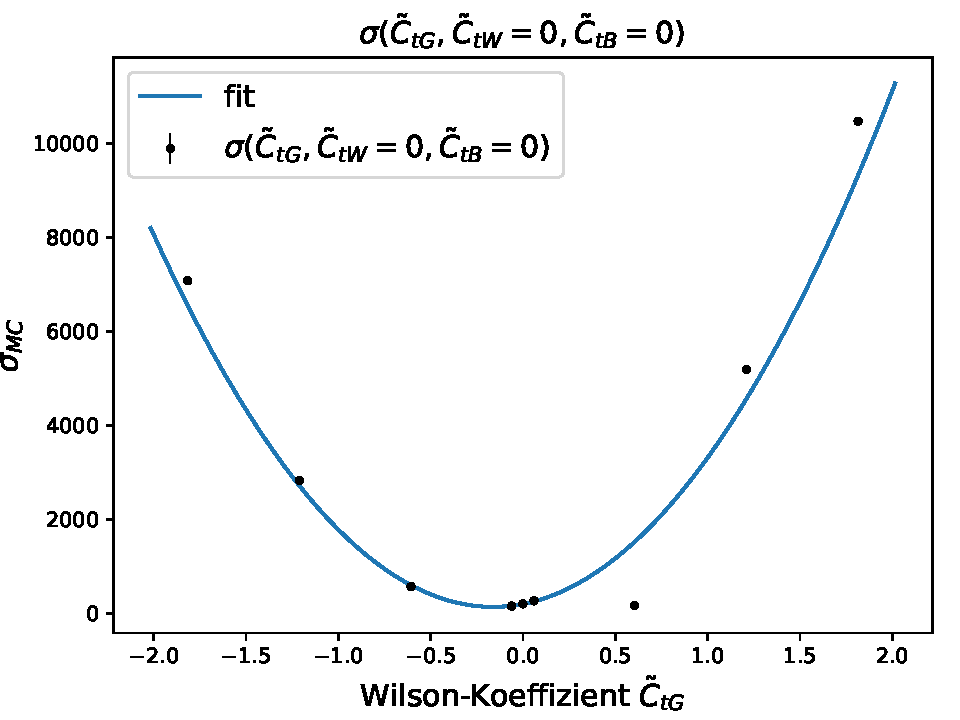
\includegraphics[width=0.5\textwidth]{Plots/combi_plot_tG.pdf}
  \caption{Graphische Darstellung des parabelförmigen Verlaufs der Wirkungsquerschnitte für den Wilson-Koeffizienten $C_{tG}$, wenn $C_{tW}=C_{tB}=0$ ist.}
  \label{fig:WtG}
\end{figure}

\section{MadGraph Modell für den EFTfitters}
Durch die Bestimmung der gesuchten Parameter mit der Methode der kleinsten Quadrate werden die folgende Wirkungsquerschnitte:
\begin{align*}
  \bar{\sigma}_{SM}   &= 202.19\\
  \bar{\sigma}_{tG} &= 21.68\\
  \bar{\sigma}_{tW} &= 21.69\\
  \bar{\sigma}_{tB} &= 761.42\\
  \bar{\sigma}_{tGtG} &= 11.79\\
  \bar{\sigma}_{tWtW} &= 11.77\\
  \bar{\sigma}_{tBtB} &= 48.44 \\
  \bar{\sigma}_{tGtW} &= 6863.76\\
  \bar{\sigma}_{tGtB} &= -6483.31\\
  \bar{\sigma}_{tWtB} &= 279.22
\end{align*}
erhalten. Die Unsicherheiten aus dem Fit mit der Methode der kleinsten Quadrate werden hier vernachlässigt. Dies liegt daran, dass sie lediglich statistische Abschätzungen sind und gewisse Annahmen beinhalten, bei denen nicht klar ist, ob sie für das betrachtete Modell aussagekräftig sind. Zudem handelt es sich um einen hochdimensionalem Fit, sodass sehr geringe Abweichungen, wie sie im Fall von $C_{tG}$ vorhanden sind, starke Auswirkungen haben.
%
%
\chapter{EFT-Interpretation des \texorpdfstring {$t\bar{t}\gamma$}{math} Produktionswirkungsquerschnitts mit dem EFTfitter}

\section{Ergebnis für die Wilson-Koeffizienten}

\begin{figure}
    \centering
    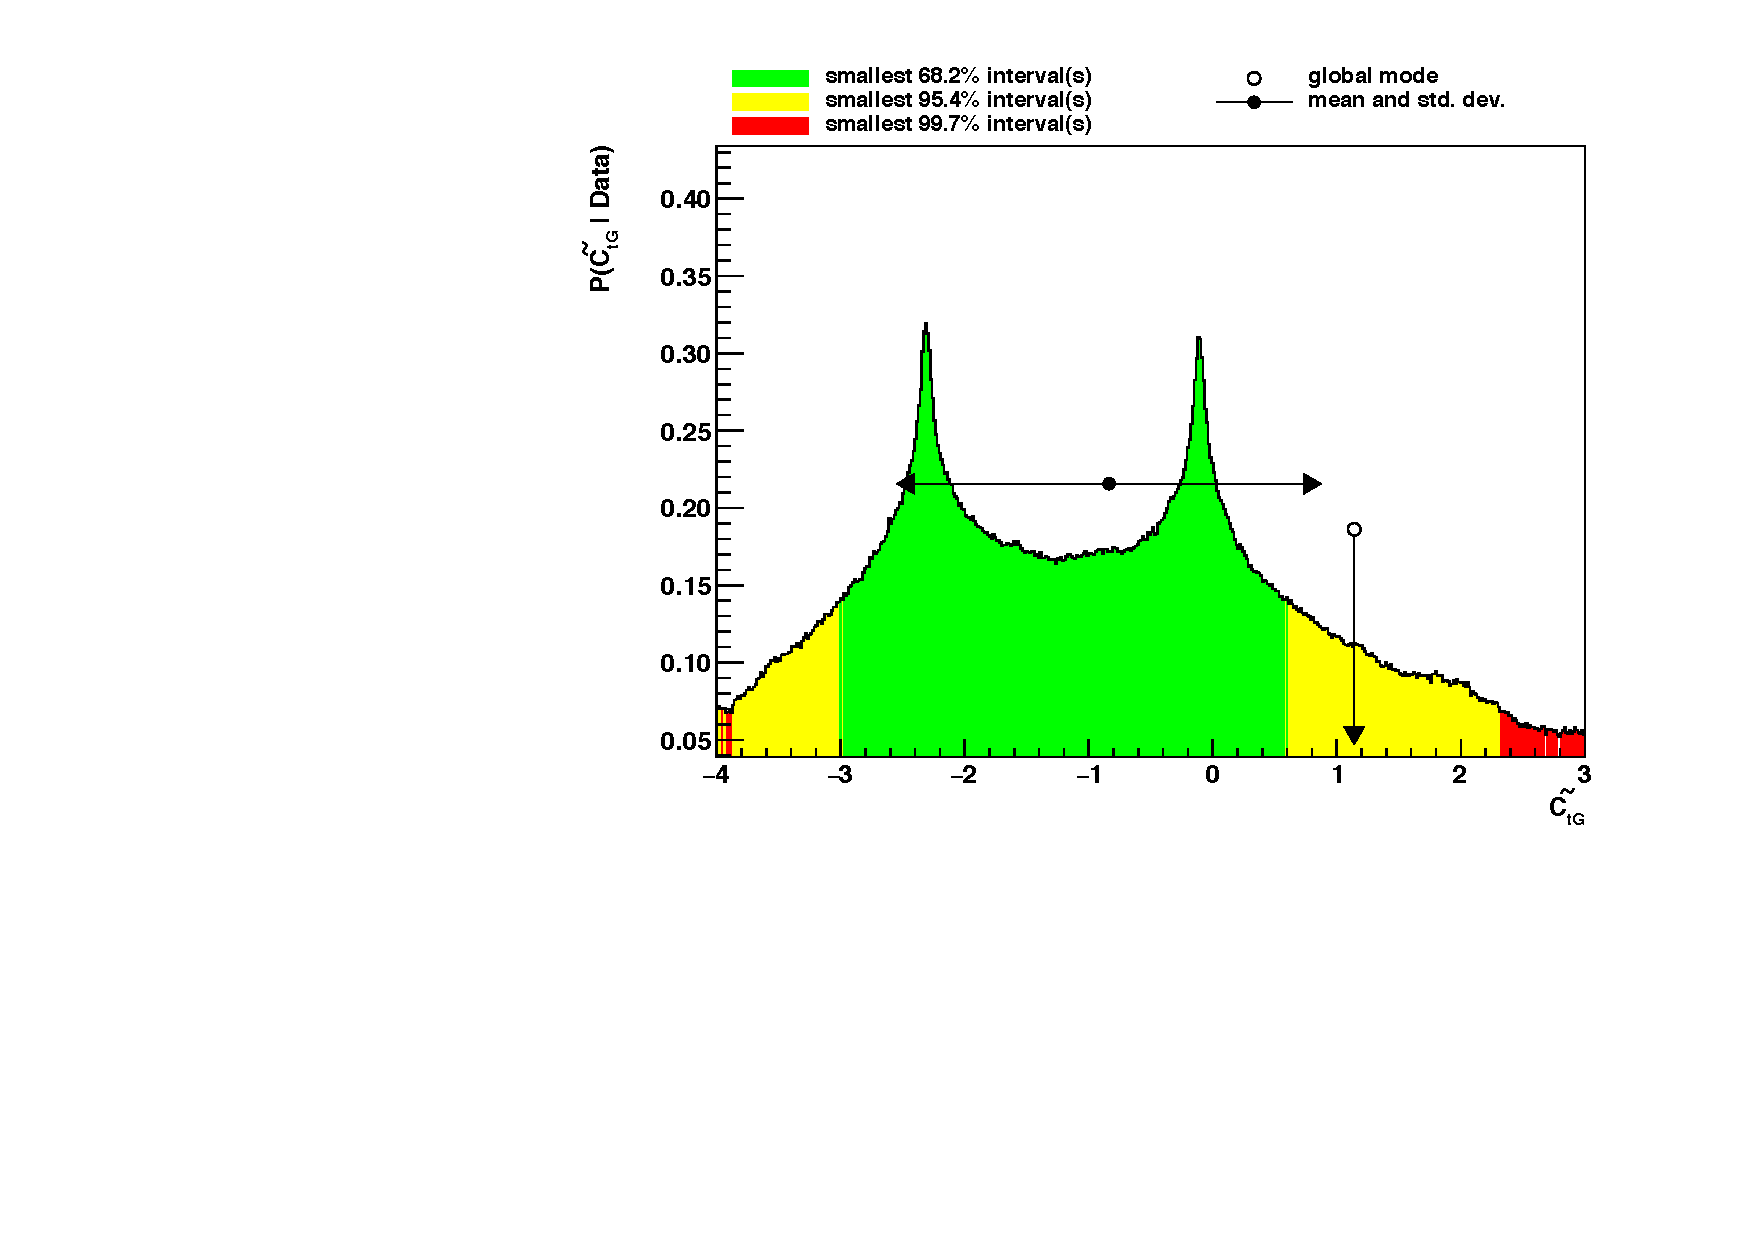
\includegraphics[width=0.8\textwidth]{Plots/result_CtG.pdf}
\end{figure}
\begin{figure}
    \centering
    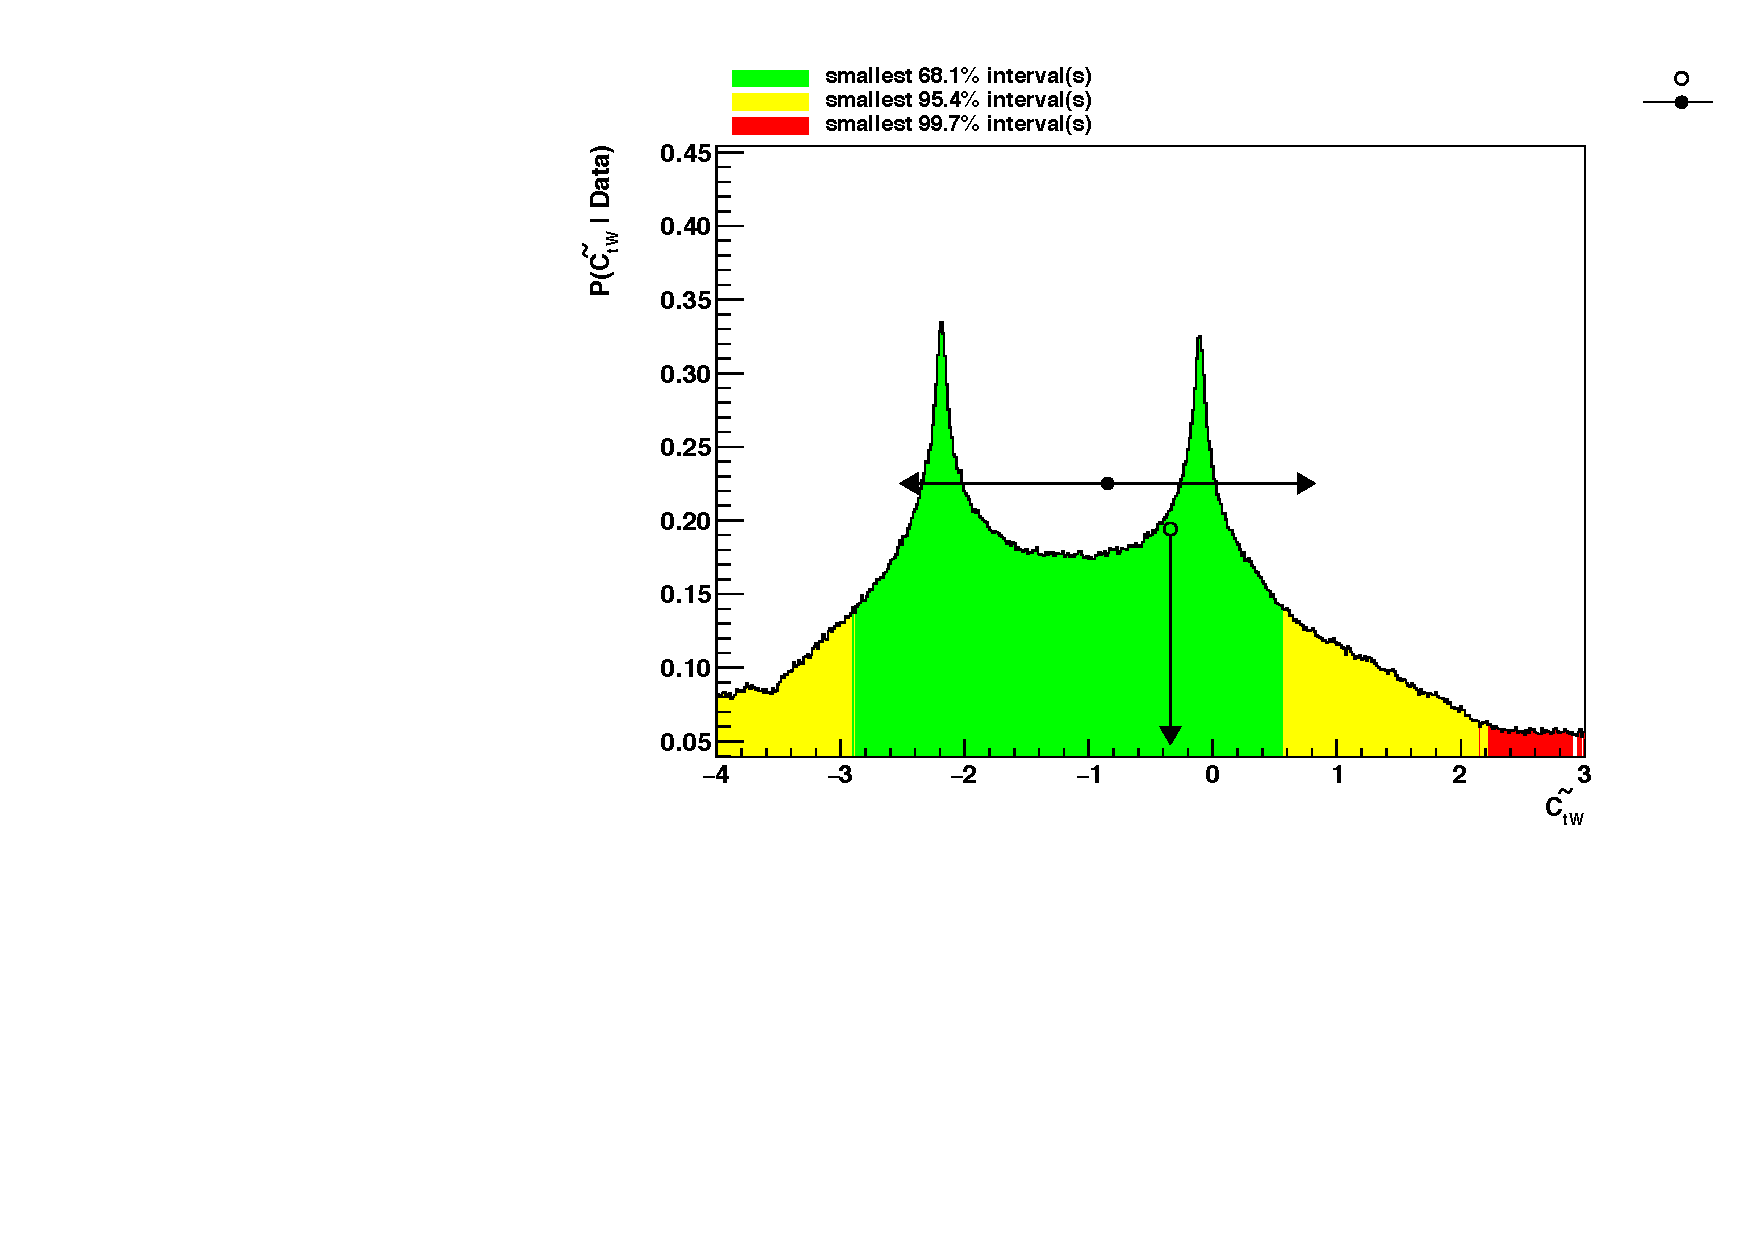
\includegraphics[width=0.8\textwidth]{Plots/result_CtW.pdf}
\end{figure}
\begin{figure}
    \centering
    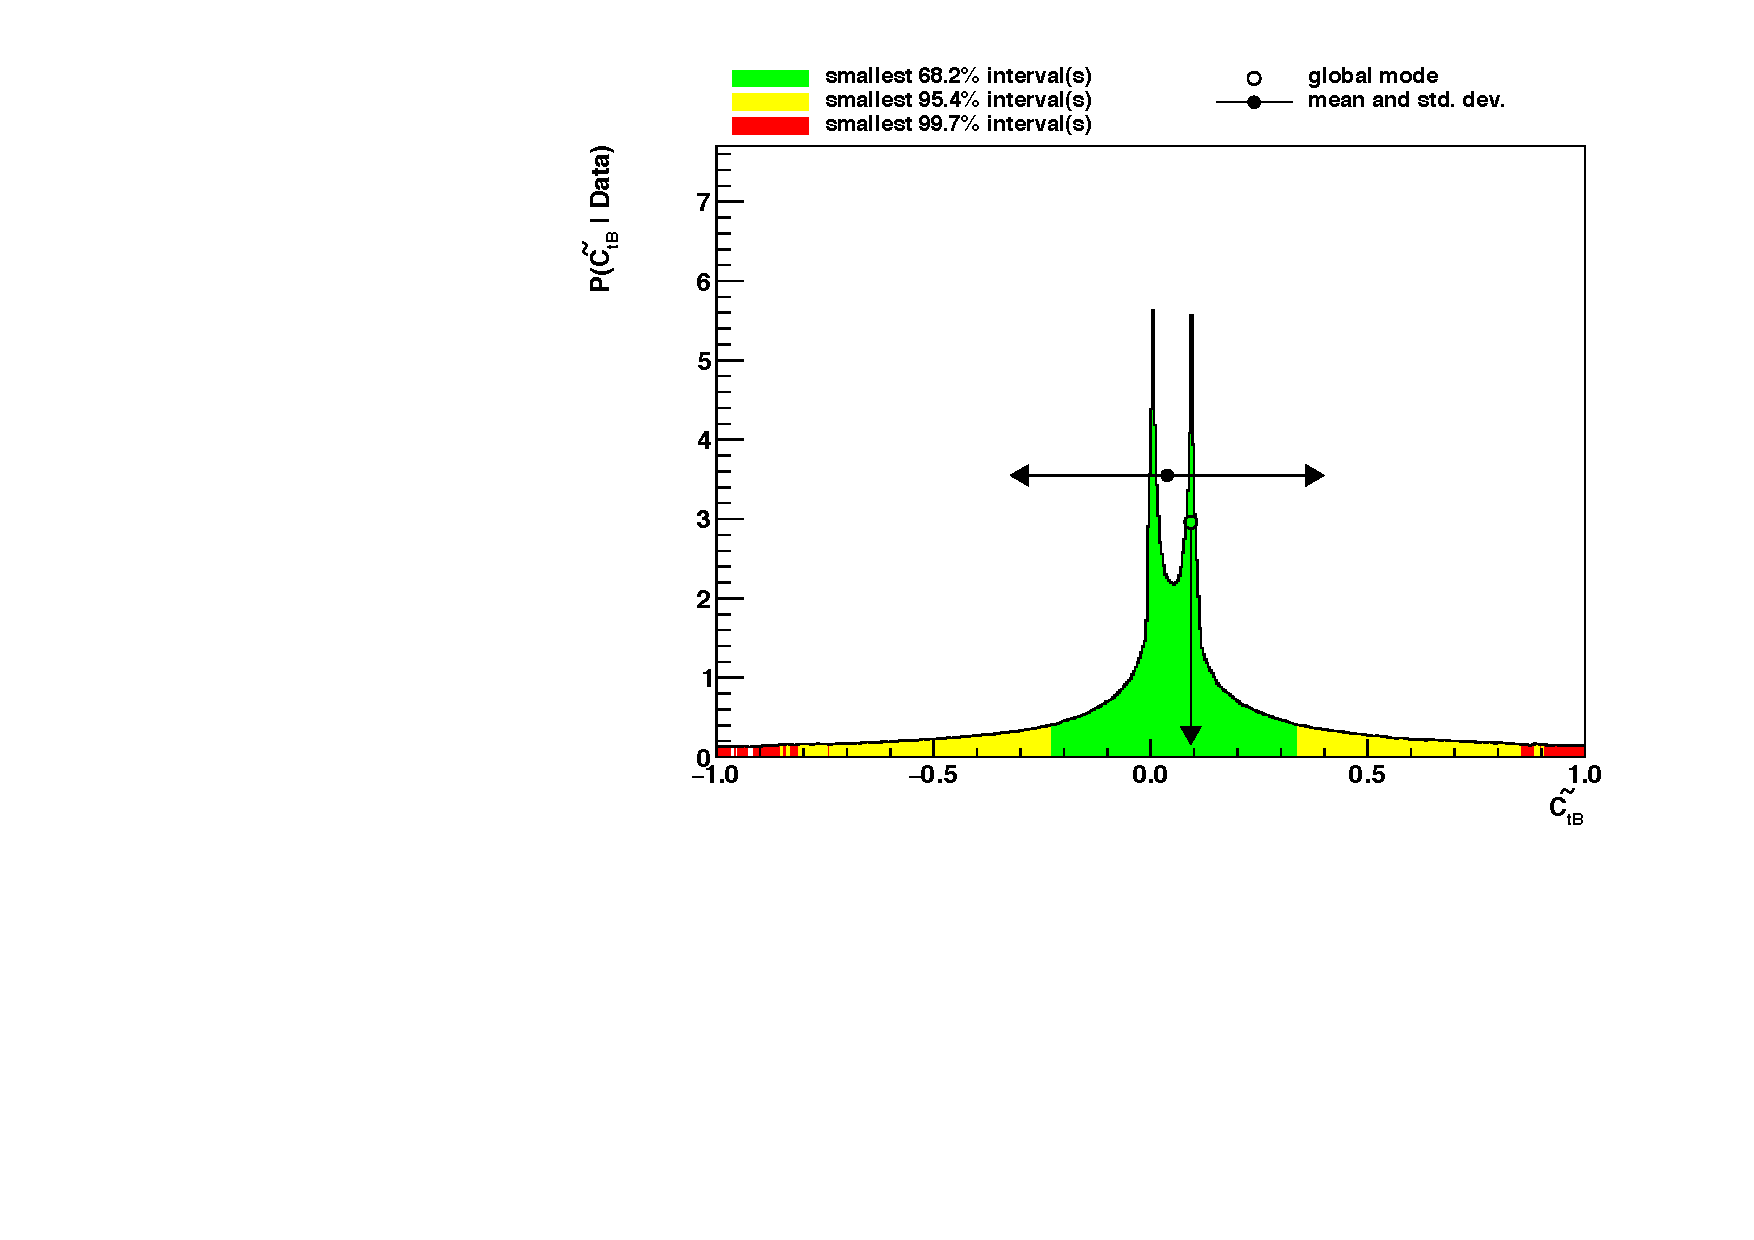
\includegraphics[width=0.8\textwidth]{Plots/result_CtB.pdf}
\end{figure}
\begin{figure}
    \centering
    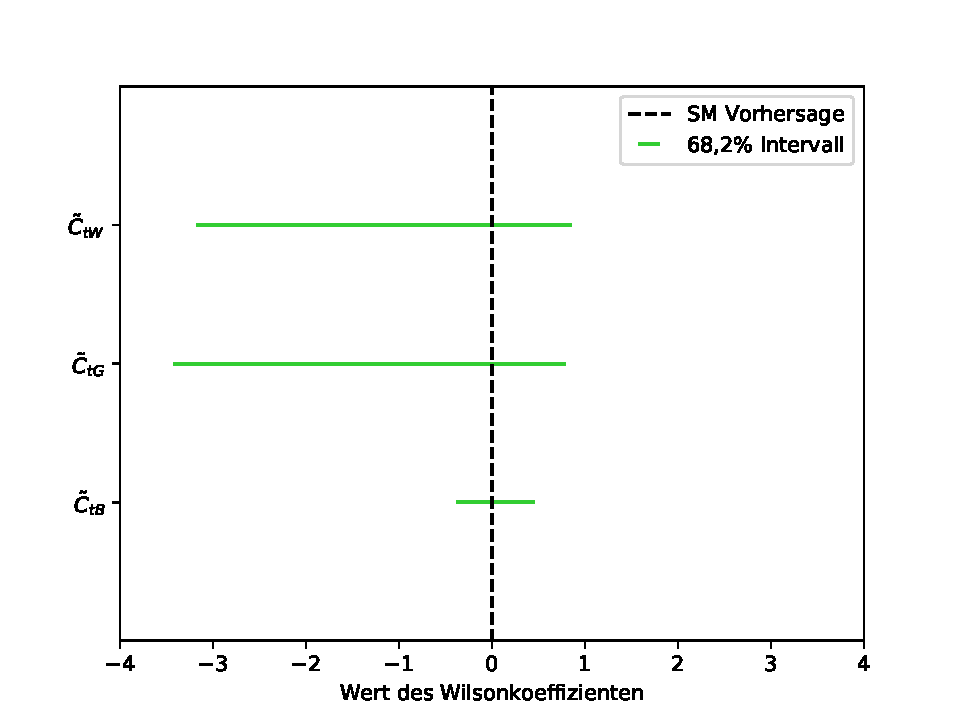
\includegraphics[width=0.8\textwidth]{Plots/wilson.pdf}
\end{figure}
%
%
\chapter{Zusammenfassung}
